%!TEX root = ../../thesis.tex
%*******************************************************************************
%****************************** Solution Implementation Chapter *********************************
%*******************************************************************************

\chapter{Solution Implementation}

\ifpdf
    \graphicspath{{Chapters/Implementation/Figs/}{Chapters/Implementation/Figs/}{Chapters/Implementation/Figs/}}
\else
    \graphicspath{{Chapters/Implementation/Figs/}{Chapters/Implementation/Figs/}}
\fi
In the previous chapter, we displayed an architectural overview of our solution approach.
Consequently, the solution implementation chapter of this thesis presents the details of how the proposed system was developed and implemented.
Firstly, we define some \ac{df} (see section \ref{implementation:section:designfeatures}) that focus on designing and developing new artifacts, methods, or systems.
Next, the description of the technology stack and development tools is explained (see section \ref{implementation:section:technologies}).
The chapter includes a detailed explanation of the critical features and functionality of the system and the processes used in frontend implementation (see section \ref{implementation:section:frontend}), database implementation (see section \ref{implementation:section:database}) backend implementation (see section \ref{implementation:section:backend}), and the software tool (see section \ref{implementation:section:tool}).
Through this chapter, readers will understand how we brought the proposed solution to reality and its potential for real-world applications.

\section{Tool Design Features (DFs)}
\label{implementation:section:designfeatures}
Our \ac{dsr} aims to produce a tangible outcome, such as a new software tool, a process improvement, or a theoretical framework with the derived \ac{df}s.
It often involves multiple cycles of design, evaluation, and redesign, allowing for constant improvement of the artifact.
Since we perform the \textit{first} iteration of the cycle, we derive the features of our software tool using the \ac{df}s.
In this section, we translate each \ac{dp}s (we defined in chapter \ref{chap:design}) into a set of \ac{df}s that we can directly implement into the tool or solution approach and we describe the \ac{df}s for each of the derived \ac{dp}s.
As shown in the figure \ref{fig:implementation:hierarchy}, we see that the \ac{df}s are divided according to the \textit{LEAN} development cycle.
\clearpage

\begin{figure}[htbp!]
    \centering
    \begin{subfigure}[b]{1.0\textwidth}
    \centering
    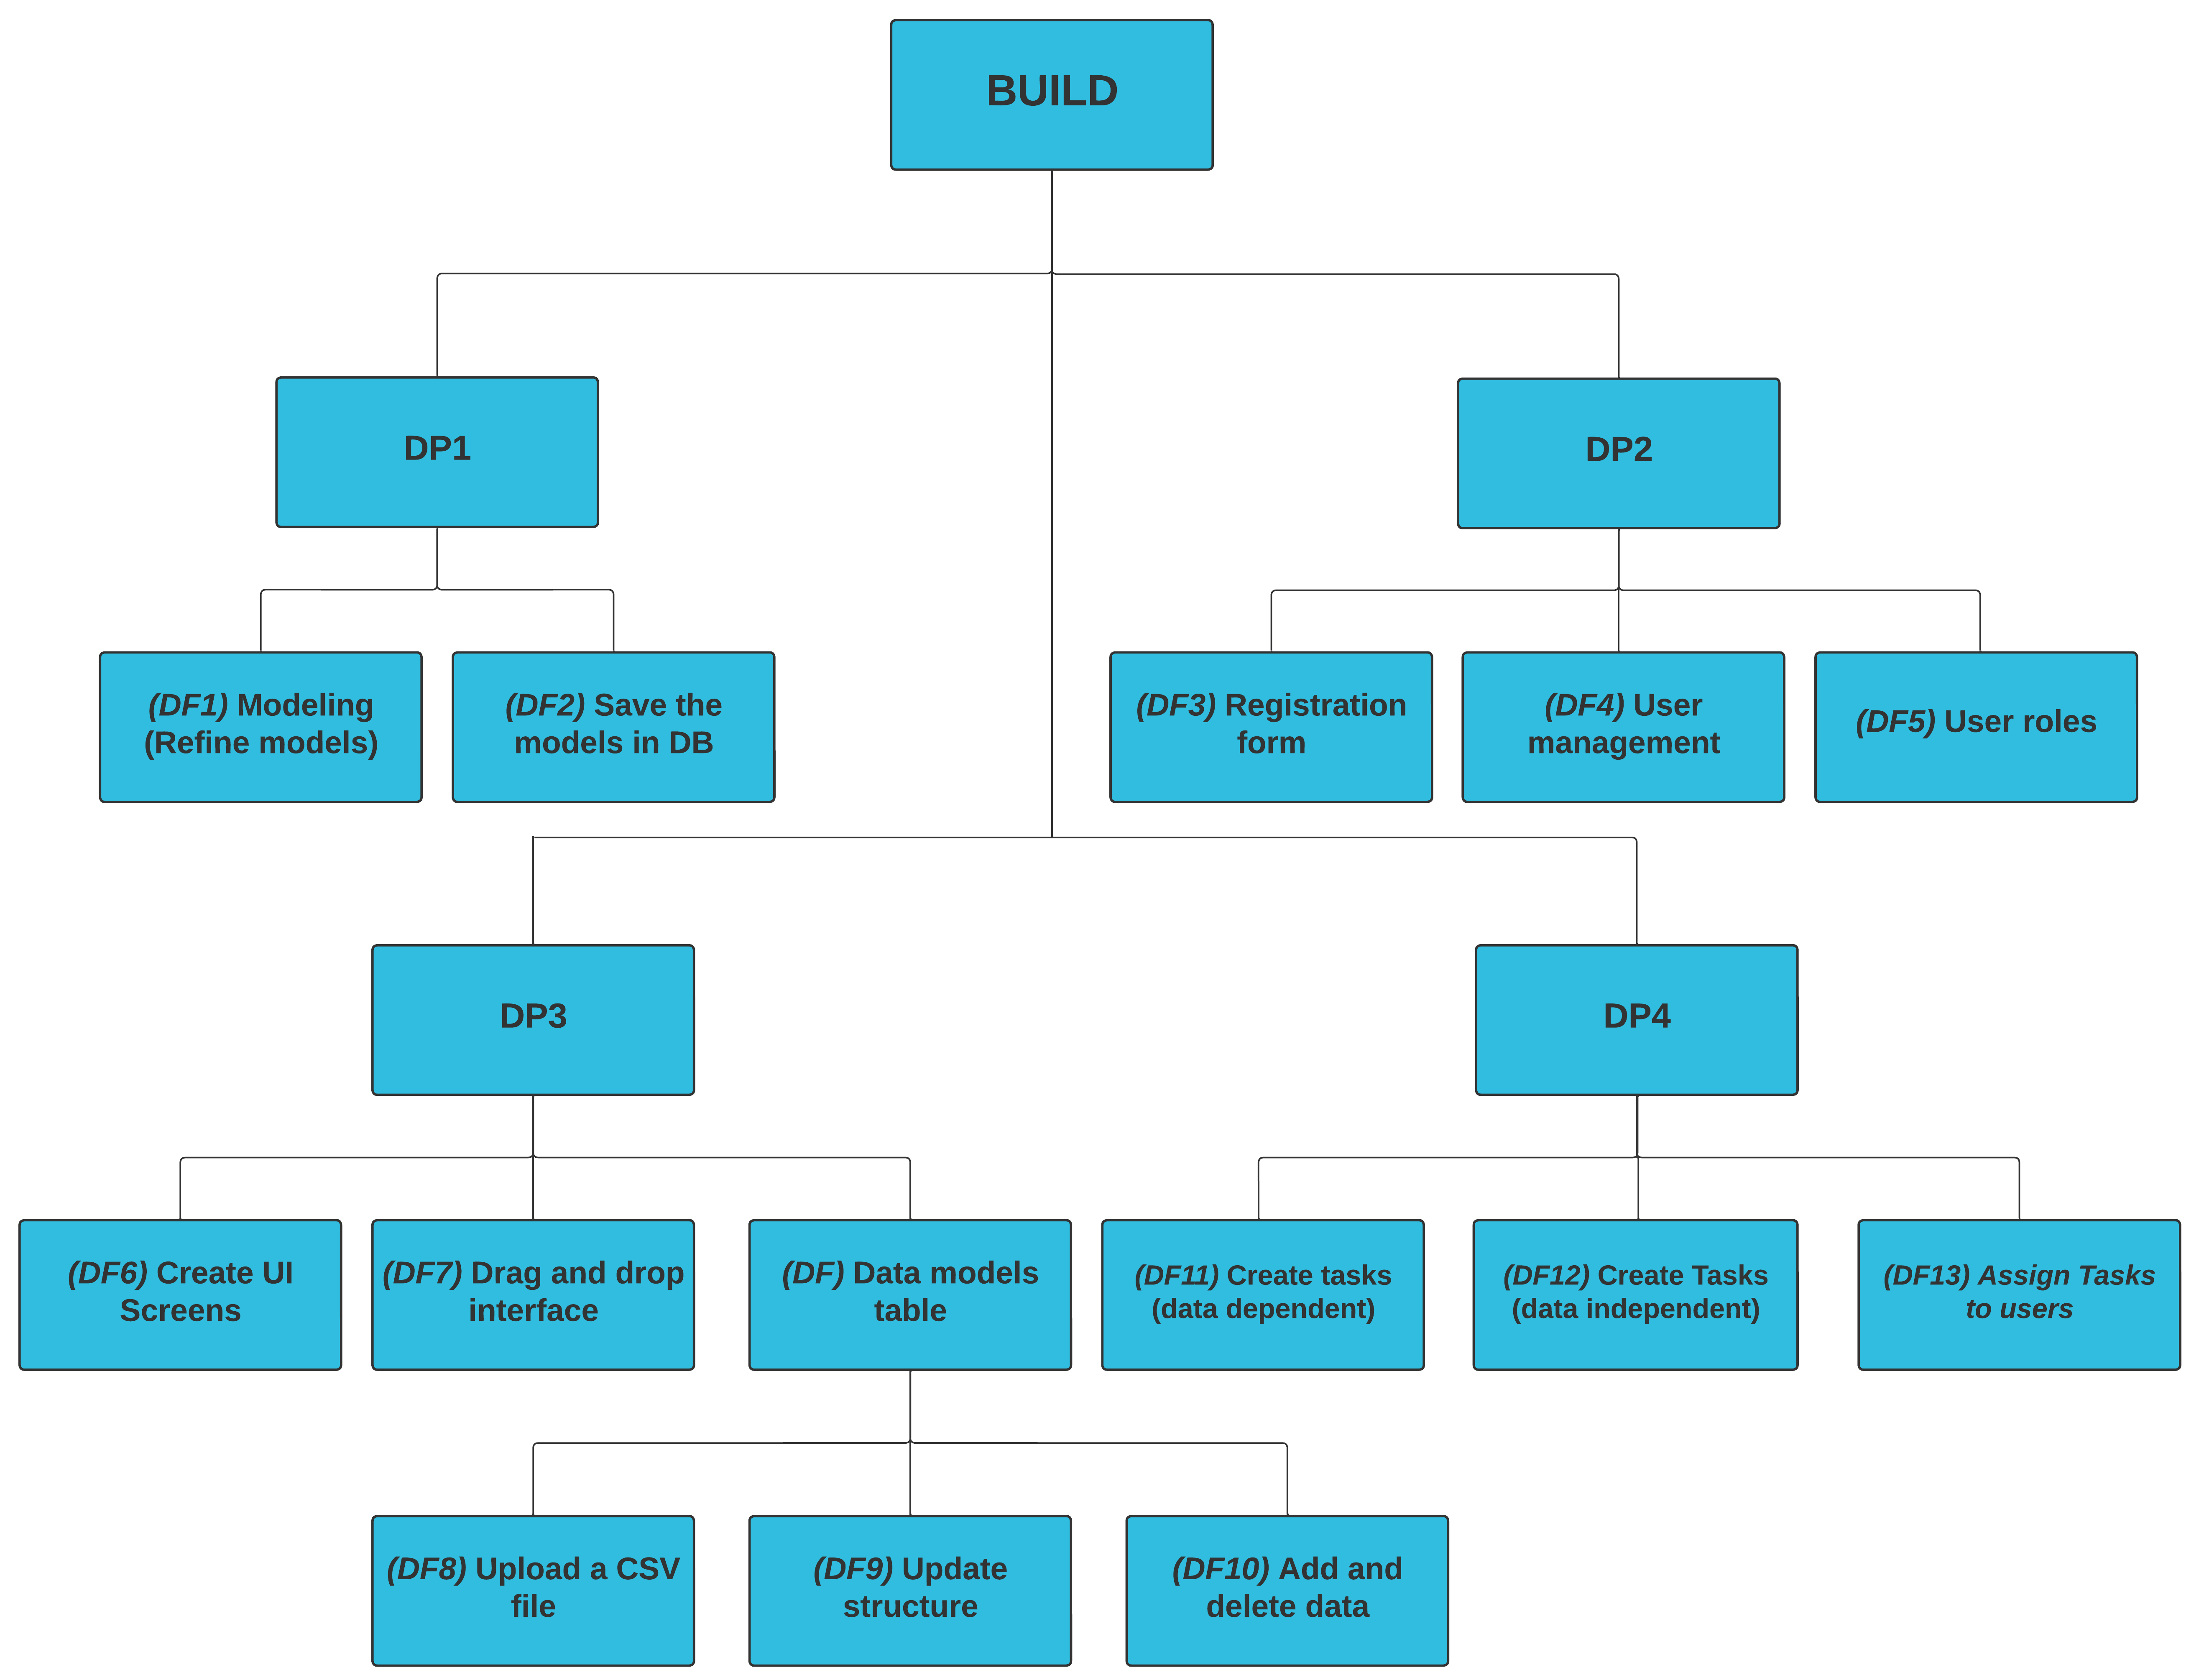
\includegraphics[width=0.8\textwidth]{DFs_hierarchy_build.png}
    \caption{A hierarchical diagram of \ac{df}s from \textit{Build} phase}
    \label{fig:implementation:hierarchy:build}
    \end{subfigure}
    \begin{subfigure}[b]{1.0\textwidth}
    \centering
    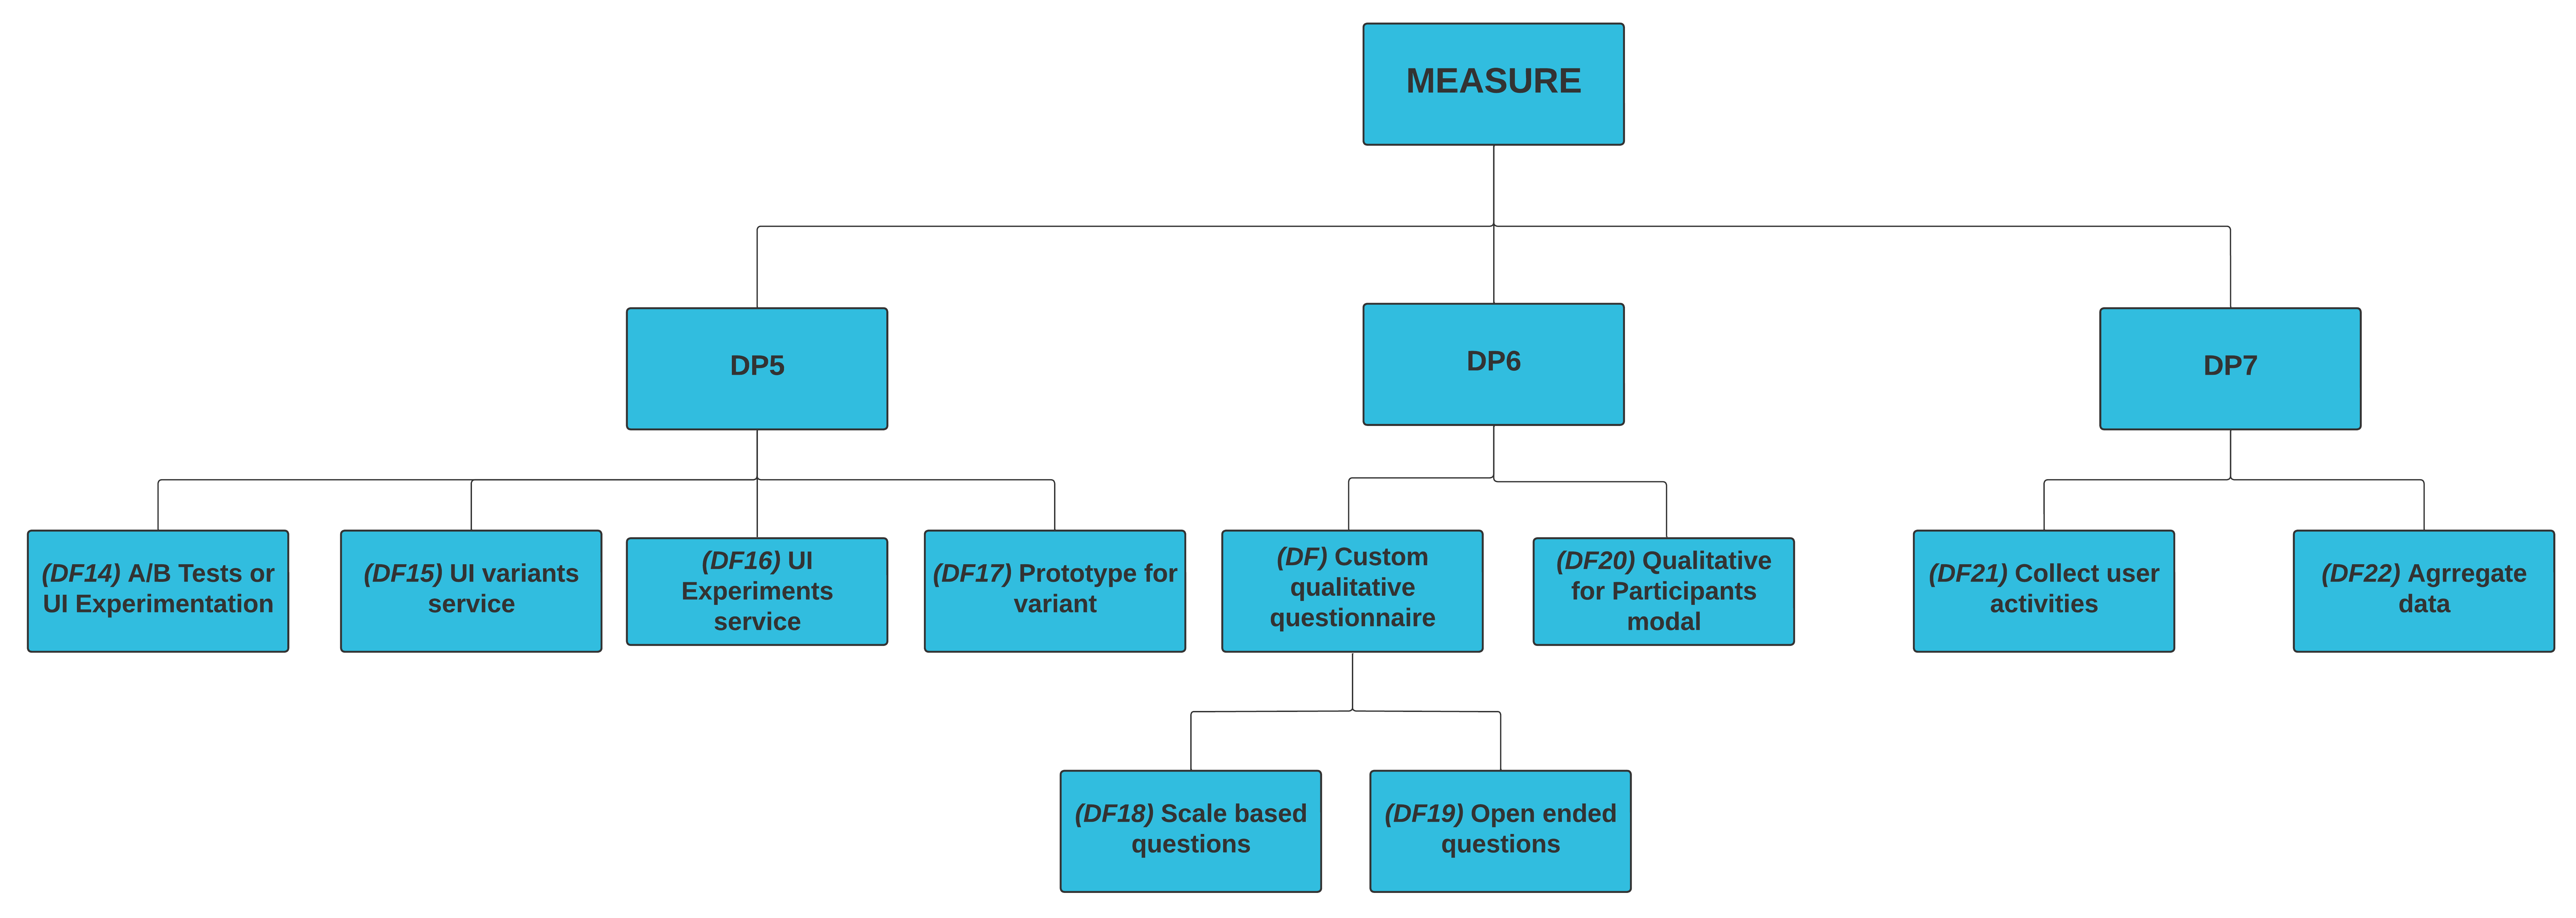
\includegraphics[width=1.1\textwidth]{DFs_hierarchy_measure.png}
    \caption{A hierarchical diagram of \ac{df}s from \textit{Measure} phase}
    \label{fig:implementation:hierarchy:measure} 
    \end{subfigure}             
    \begin{subfigure}[b]{0.8\textwidth}
    \centering
    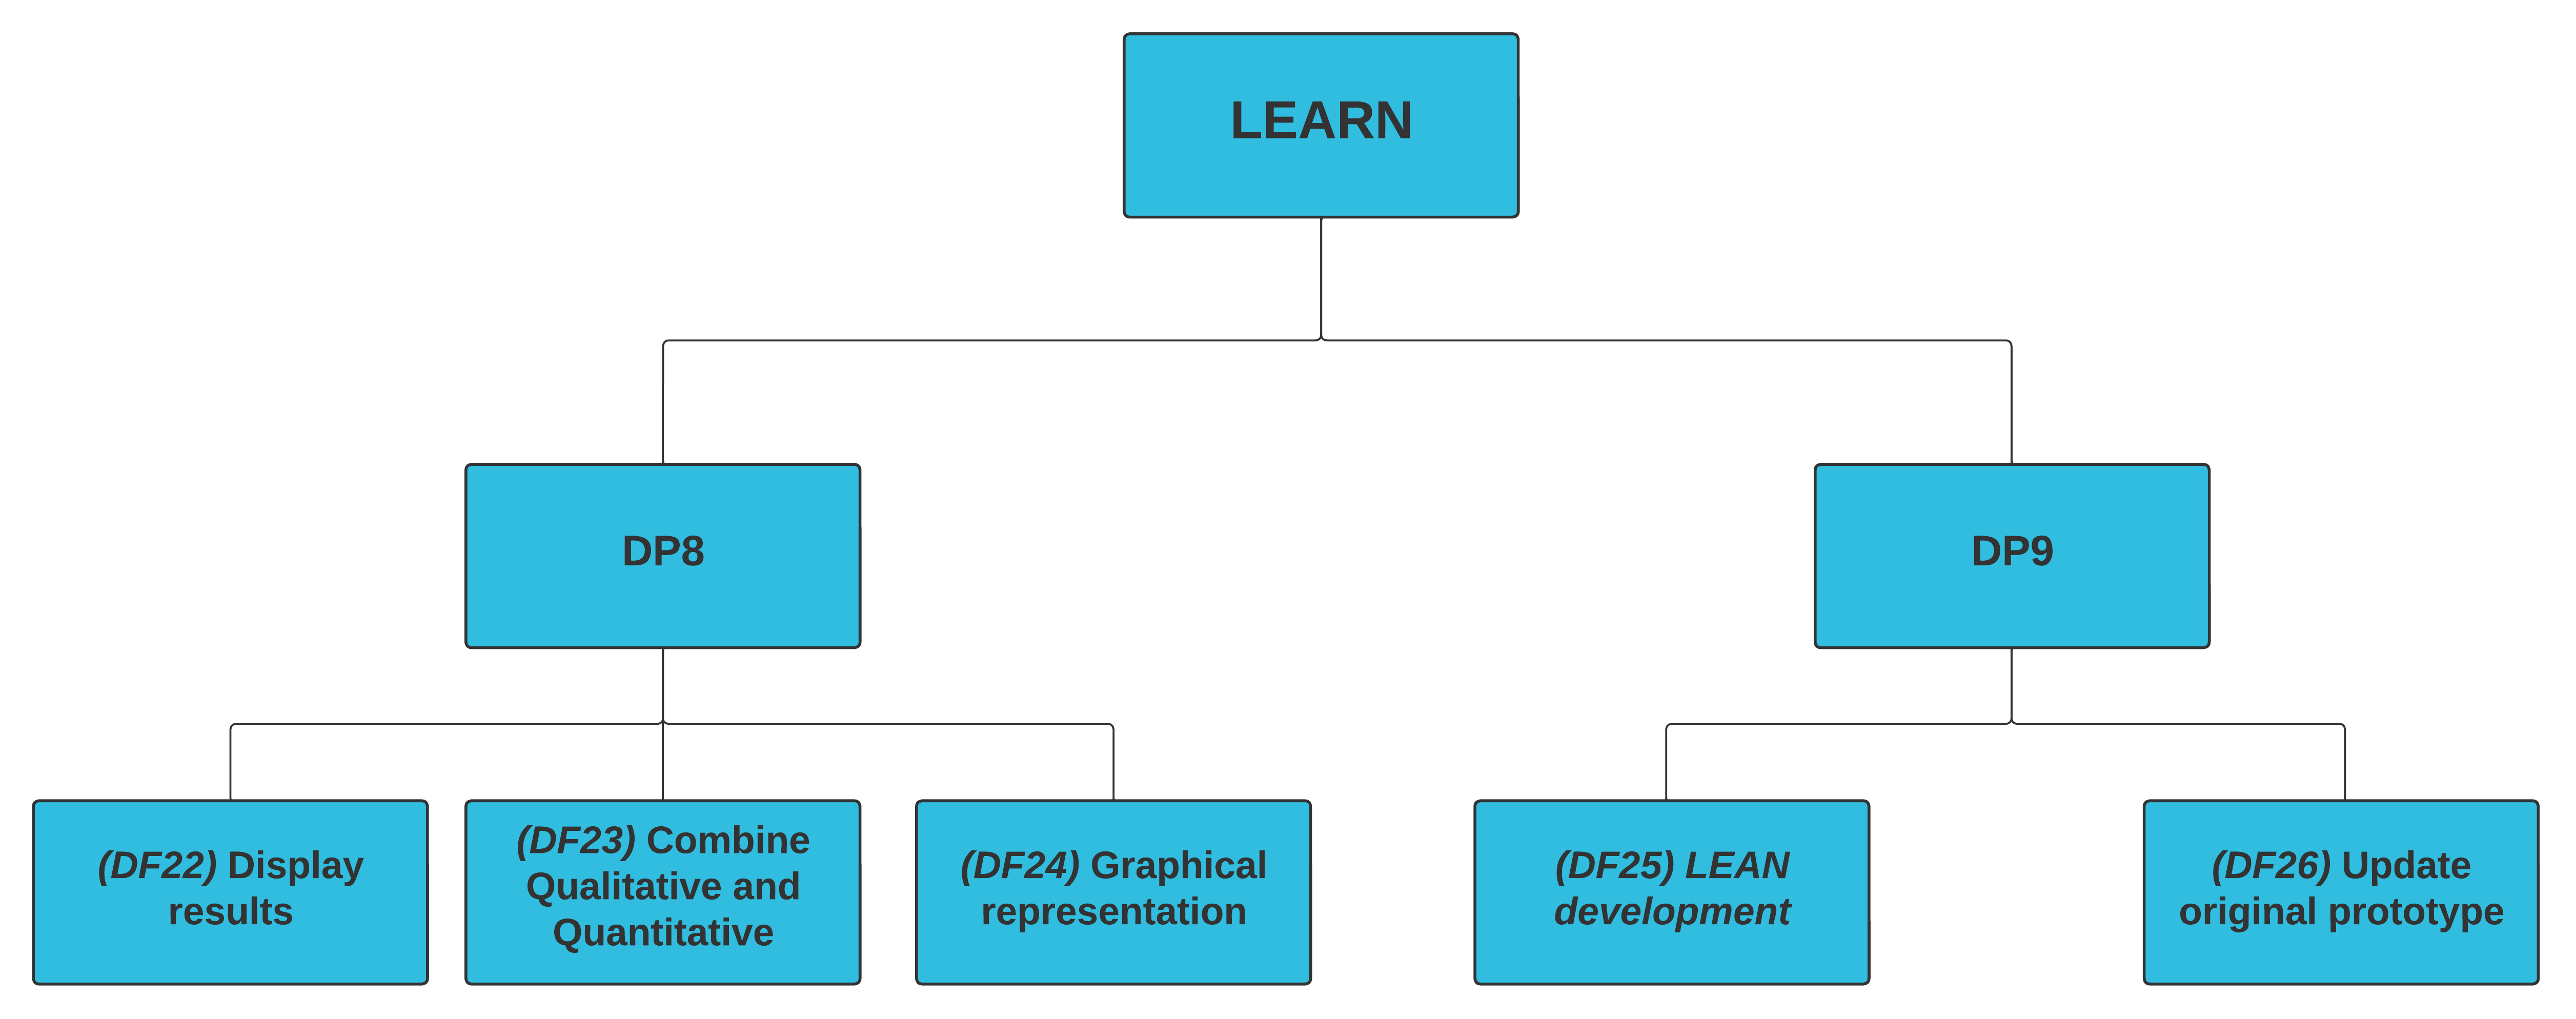
\includegraphics[width=1.0\textwidth]{DFs_hierarchy_learn.png}
    \caption{A hierarchical diagram of \ac{df}s from \textit{Learn} phase}
    \label{fig:implementation:hierarchy:learn}
    \end{subfigure}
    \caption[A map between \ac{dp}s and \ac{df}s]{Hierarchical structure of \ac{df}s}
    \label{fig:implementation:hierarchy}
\end{figure}
\paragraph{Build:}
In the \textit{Build} phase of the \textit{LEAN} development cycle, based on the \textbf{\ac{dp}1: Modeling}, the solution tool provides features for creating the models (\textit{\ac{df}1}) useful for persisting data in the database and updating them (\textit{\ac{df}2}) by iterating and improving the models with the results of the experiments.
It helps to create our prototypes in a model-based approach and improve our prototypes by improving the models throughout the LEAN development cycle.
With the \textbf{\ac{dp}2: User Variety}, the key features of our solution tool for the \ac{ui} prototyping tool will include registration for diverse users using a registration form (\textit{\ac{df}3}) and user management, i.e., features that enable team members to create and manage user accounts (\textit{\ac{df}4}), assign different levels of access and permissions (\textit{\ac{df}5}).
The \textit{User module} maintains all these features and also the user authentication, authorization, and user profile management.
Next, based on the \textbf{\ac{dp}3: Flexible UI Elements}, the privileged user prototypes using the features of our solution tool, which includes the creation of different screens (\textit{\ac{df}6}) and reusable \ac{ui} elements using a drag and drop interface (\textit{\ac{df}7}). 
The tool also provides a feature to add custom data i.e., creating data models by uploading a \ac{csv} file (\textit{\ac{df}8}), revising structures of data model table (\textit{\ac{df}9}), adding and deleting data from the table (\textit{\ac{df}10}).
Next, based on the \textbf{\ac{dp}4: User tasks Refinement}, the privileged user creates \textit{User Tasks} for the users using the features of our solution tool, which includes creating tasks for users depending on the data model (\textit{\ac{df}11}) and independent of data models (\textit{\ac{df}12}), and assign the task to the experiments (\textit{\ac{df}13}).

\paragraph{Measure:}
In the \textit{Measure} phase of the \textit{LEAN} development cycle, based on the \textbf{\ac{dp}5: Split Tests}, the privileged user would be able to create A/B tests or \ac{ui} experimentation (\textit{\ac{df}14}) using the features of our solution tool, which includes creating and modifying the experiments (\textit{\ac{df}15}), creating and updating the \ac{ui} variants (\textit{\ac{df}16}), and modifying the variants' prototypes such that each variant has a unique view (\textit{\ac{df}17}).
Next, based on the \textbf{\ac{dp}6: Qualitative Analysis}, the privileged user would be able to do qualitative analysis on the users using the features of our solution tool, which includes creating the custom qualitative questionnaire with options in the answering formats like \textit{Scale based}, i.e., the users will have to choose from options 1 to 10 (\textit{\ac{df}18}) and open-ended questions, i.e., the users will have the freedom to answer whatever they think (\textit{\ac{df}19}). 
And, the user participants will answer these qualitative questions after finishing the tasks with a modal appearing with different questions (\textit{\ac{df}20}). 
Similarly, based on the \textbf{\ac{dp}7: Quantitative Analysis}, the privileged user creates quantitative analysis on the users using the features of our solution tool, which includes collecting the task data feedback, i.e., collecting the time taken to finish the task, number of unsuccessful attempts, the path taken by the users to complete the task, etc. (\textit{\ac{df}21}), and aggregating these feedback data (\textit{\ac{df}22}). 

\paragraph{Learn:}
In the \textit{Learn} phase of the \textit{LEAN} development cycle, based on the \textbf{\ac{dp}8: Diversity in Analysis}, the privileged user compares the statistics using the features of our solution tool, which includes showing the results of the experiment (\textit{\ac{df}23}), combining qualitative and quantitative analysis of each variant (\textit{\ac{df}24}), and a graphical view to see the results (\textit{\ac{df}25}). 
Finally, based on the \textbf{\ac{dp}9: Continuous Design}, the solution tool would provide features including LEAN development cycle (\textit{\ac{df}26}). 
The privileged user should be able to update the original prototype with the results from the experiment (\textit{\ac{df}27}) for continuous improvement.

Overall, the design features section in DSR delivers a comprehensive overview of the solution tool to address the identified problem or research question. 
Moreover, this section describes the \ac{df}s for our \ac{poc} solution tool.
\clearpage

\section{Software Tool}
\label{implementation:section:tool}

\clearpage
\section{Technologies Used}
\label{implementation:section:technologies}
We have created a software tool that allows us to test the features (\ac{df}s) and underlying principles of the developed DFs with actual users.
To test our solution approach, we developed a rapid prototyping tool for the first cycle of our \ac{dsr}. 

The implementation of our \textit{UI Prototyping Tool with Experimentation (UPTE)} uses various technologies.
Our UI prototyping tool was developed using Angular\footnote{A framework of javascript: \url{https://angular.io/}}, Loopback\footnote{A framework of the NodeJS \url{https://loopback.io/}}, and MongoDB\footnote{A non-relational database \url{https://www.mongodb.com/}}.
Angular is a JavaScript framework used for building web-based applications.
It provides comprehensive tools for creating dynamic and responsive UI components and handling user interactions.
With angular, we are using several other UI components which are available on Node package manager (npm)\footnote{NPM: \url{https://www.npmjs.com/}}.

Loopback is a Node.js\footnote{NodeJS: \url{https://nodejs.org/en/}} framework used for building RESTful APIs. 
It provides an intuitive interface for creating API endpoints and managing data persistence. 
Loopback's support for various data sources, including relational and NoSQL databases, makes it a versatile choice for web applications. 
We connect our database using the data managers provided by the loopback framework.
The framework's ability to generate API documentation and testing tools simplifies our development process.

MongoDB is a NoSQL document-oriented database used for storing unstructured data. 
We store our prototyping tool's data using a JSON\footnote{What is JSON: \url{https://developer.mozilla.org/en-US/docs/Glossary/JSON}} format in an unstructured manner.
It provides a scalable and flexible solution for managing volumes of data. 
MongoDB's support for automatic sharding and replication ensures high availability and fault tolerance. 
The database's dynamic schema and rich query language make it easy to adapt to changing data requirements.

By leveraging these technologies, our UI prototyping tool delivered a powerful and user-friendly interface while ensuring efficient data retrieval and storage.
Based on these technologies, we build a microservice architecture explained in the next section so that our \ac{dp}s and \ac{df}s can be easily implemented. 
\clearpage

% \section{Solution Architecture}
% \label{implementation:section:architecture}

\section{Frontend Implementation}
\label{implementation:section:frontend}

This section discusses the front-end implementation of our software tool. 
As discussed in the previous section, we developed the \ac{ui} using \textit{Angular}, a popular front-end framework. 
Angular provides a comprehensive architecture (see figure \ref{implementation:fig:angulararchitecture}\footnote{Fig taken from: \url{https://www.geeksforgeeks.org/angular-7-architecture/}}) that includes components, templates, event binding, property binding, directives, and injectors. 
Angular's architecture is organized into modules containing specific functions designed to achieve particular goals. 
These modules can be imported and exported between different Angular applications. 
In each application, a root module is launched at the start of the application and imports other modules to add additional functionality.

\begin{figure}[ht]
    \centering
    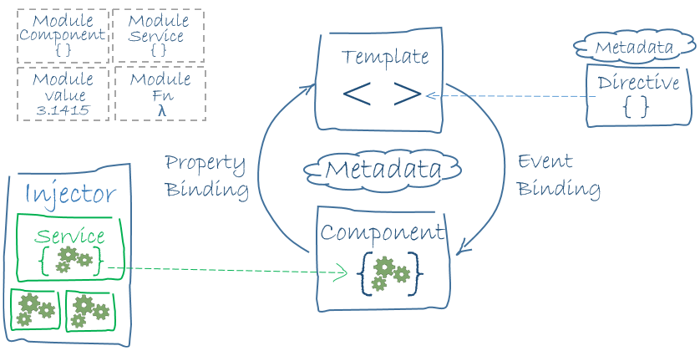
\includegraphics[scale=0.5]{angular-architecture.png}
    \caption[Angular Architecture]{Angular Architecture}
    \label{implementation:fig:angulararchitecture}
\end{figure}

In our implementation, the angular application has a root entry point, a module file (see Listing \ref{listing:implementation:allmodule}), containing all the necessary imports to function properly. 
Within our NgModule, we have imported various user-developed modules and third-party modules like \textit{MatInputModule}, \textit{NgxMatFileInputModule}, and \textit{DragDropModule} for UI elements. 
By importing these modules, we can utilize their functions and features within our application to enhance its overall functionality and user experience.
We are also using \textit{Angular Material Design}\footnote{Website for Angular material design: \url{https://v7.material.angular.io/}} which is providing a library of pre-built UI components that follow Material Design guidelines, such as buttons, forms, and navigation menus. 
It saves time designing and developing UI elements from scratch and instead focuses on customizing them to fit our needs.
\textit{Nginx File Input}\footnote{Website for Angular Material File Input \url{https://www.npmjs.com/package/@angular-material-components/file-input}} is another third-party module we have imported into our application. 
This module allows users to upload files directly from their local device, enabling us to save them to our server for future use.
Finally, the \textit{Drag and Drop module}\footnote{Website for the Angular material Drag and drop \url{https://v7.material.angular.io/cdk/drag-drop/api}} allows users to easily rearrange elements on the \ac{ui} by dragging and dropping them to their desired location. 
Utilizing this module can provide a more interactive and dynamic user experience for prototyping.

\begin{lstlisting}[language=JavaScript, caption=all-component.module.ts, label=listing:implementation:allmodule]
// Components
import { LoginComponent } from './components/login/login';
...
// Modules
import { DragDropModule } from '@angular/cdk/drag-drop';
import { AppRoutingModule } from '../app-routing.module';
import { NgxMatFileInputModule } from '@angular-material-components/file-input';
// Material design
import { MatSidenavModule } from '@angular/material/sidenav';
...

@NgModule({
    declarations: [
        LoginComponent,
        ...
    ],
    imports: [
        DragDropModule,
        AppRoutingModule,
        NgxMatFileInputModule,
        MatSidenavModule,
        ...
    ],
    exports: [
        LoginComponent, 
        ...
    ]
})
export class AllComponentModule { }  
\end{lstlisting}

Our implementation focuses on the \ac{mvc} architecture, which contains services and directives to talk to the server and some middleware to add a user token to every request to authenticate the user. In the next section, we explain how we implemented the \textit{UI Prototyping component}.
In this section, we explain as an example the implemented \textit{left-panel}, \textit{middle-panel}, and \textit{right-panel} components. 
Similarly, we use the \textit{observer pattern}\footnote{Website for Observer pattern: \url{https://refactoring.guru/design-patterns/observer}} for the interaction between these components and various services to interact with the server.

\begin{lstlisting}[language=JavaScript, caption=left-panel.component.ts, label=listing:implementation:left]
import { NestedTreeControl } from '@angular/cdk/tree';
import { Component, OnInit } from '@angular/core';
...
@Component({
    templateUrl: './left-panel.component.html',
    ...
})
export class LeftPanelComponent implements OnInit {
    // Define variables ...
    constructor(private shared: CommunicationService, private viewService: ViewsService, ...) { }

    async ngOnInit() {
        // get master view from server
        let master: View = await firstValueFrom(this.viewService.getMasterView())
    }

    // CRUD of view
    addView(isMaster: boolean = false, node: View = new View()) {
        let master: View = this.dataSource.data[0]
        master.children.push(View.getView(false, name))
        this.dataSource = new MatTreeNestedDataSource<View>()
    }
    ...

    // Emit events and the other panels/components capture them
    addElement(elementName: string) {
        this.shared.setAddUIElement(elementName)
    }

}    
\end{lstlisting}
\paragraph{Left panel}
The left-panel component contains a list of UI elements that can be added to the screen.
It allows users to navigate and manipulate the elements on the screen easily, improving the \ac{ux}.
In our implementation (see Listing \ref{listing:implementation:left}), firstly, we added a \texttt{@Component} decorator to the component's TypeScript file to specify the location of its template file, CSS file and selector.
Next, we added a function that fetches the master view, if present in the database, and assigns it to a variable in the component's code. 
This function is called during the initialization of the component called \texttt{ngOninit}. 
We also included functionality for CRUD operations for the views or UI screens in the prototyping phase. 
It includes adding, editing, deleting, and viewing views or UI screens. 
Finally, we had several functions that emit events to other panels or components that are listening to these events. 
It allows for communication and coordination between different parts of the application.
Similarly, the \textit{template} of the left panel contains a tree structure that displays the views and their children. 
This structure allows users to easily navigate through different UI screens and select the one they want to work on. 
The left panel template also contains various UI elements that the user can add to the UI screen in the middle panel.
We have grouped them into different categories based on functionality, such as form elements, buttons, text elements, etc. 
Each category can be expanded or collapsed to make it easier to find the desired element.

\paragraph{Middle Panel}
In our implementation, firstly, in the constructor, the middle panel component (see Listing \ref{listing:implementation:middle}) creates a renderer to listen to mouse and keyboard events.
This component subscribes to the required events that are emitted by other components. 
For example, it listens to adding UI elements from the left panel component. 
After the event is subscribed it adds the required UI element to the screen using the \texttt{addUIElement()} method and the provided information.
It then uses the \textit{Drag API} to make the element draggable within the virtual screen and adds various listeners.
When the element is moved and placed at a certain position, the draggable interface provides the element's position, which is then added to the data structure of the current element.  
This component also provides CRUD functionality for the UI elements, i.e. to add, update, and remove elements.
For instance, it adds listeners for the keyboard events, such as delete or backspace key press, and removes the element from the screen when the event is triggered.
Similarly, we implemented a \textit{template} for the middle panel component that allows the user to build the prototype visually. 
The template is designed to provide a virtual screen for the user to place UI elements. 
It contains a box that defines the dimensions of the screen and displays the name of the current view that is being edited. 
The user can place UI elements within the box by dragging and dropping them onto the screen. 
These elements are provided by the left panel component and can be customized using the properties panel component on the right. 
The middle panel component subscribes to events emitted by the left and right panel components, allowing it to update the screen in real-time.

\begin{lstlisting}[language=JavaScript, caption=middle-panel.component.ts, label=listing:implementation:middle]
@Component({...})
export class MiddlePanelComponent implements OnInit {
    // Define variables
    @ViewChild('cardContent') el!: ElementRef
    ...
    constructor(private rf:RendererFactory2,private drag:DragDrop) {
        this.renderer = this.rf.createRenderer(null, null);
    }
    async ngOnInit() {
        // Subscribe to events e.g. add UI element
        await firstValueFrom(this.shared.getAddUIElement())
        this.addUIElement()
    }
    addUIElement() {
        // Define Component
        let component: ComponentContainer = new ComponentContainer()
        component.name = this.toAddElement
        ...
        // Make it draggable
        let dragRef: DragRef = this.drag.createDrag(recaptchaContainer).withBoundaryElement(this.el)
        // Add Element, push to array, add listener
        const text = this.renderer.createText(this.toAddElement)
        this.elementsOnCanVas.push(component)
        this.addListener(recaptchaContainer, component)
        this.getPosition(dragRef, component.id)
        ...
    }
    async getPosition(dragRef: DragRef, id: string) {
        const val = await firstValueFrom(dragRef.ended)
        toAdd.cssProperty.dropPoint = dragRef.getFreeDragPosition()
    }
    async addListener(elm: Element, el: ComponentContainer) {
        // Delete the element 
        const event = await this.renderer.listen(elm, 'keydown')
        if (event.key == 'Delete' || event.key == 'Backspace') {
            elm.remove() ...
        }
    }
}
\end{lstlisting}

\paragraph{Right Panel}
In our implementation, the right panel component serves as a property editor for the selected UI element in the middle panel. 
It contains various functions which are explained using the Listing \ref{listing:implementation:right}.
It listens to events emitted by the left panel and middle panel components to update the selected element's properties. 
It also listens to events to edit the canvas or screen and to delete the element from the canvas.
The right panel contains various input fields and dropdowns to edit the properties of the selected UI element, such as color, text, font, size, etc. 
When the user selects an element on the canvas, the right panel updates with the properties of that element. 
Similarly, when a new UI element is added to the canvas, the right panel displays the default properties for that element.
Additionally, the right panel contains a function for adding new interactions to the UI element, such as \texttt{onClick} event. 
This function allows the user to define a JavaScript function that will be executed when the UI element is clicked. 
The function can be added to the element's properties in the right panel and saved to the database along with the other properties.
Moreover, the template of the right panel component displays the properties of a selected UI element. 
It is dynamically updated based on events emitted by the middle panel component. 
When the middle panel emits an event to update the selected element, the right panel template displays the properties of that element. 
Similarly, when the middle panel emits an event to update the canvas or screen, the right panel template updates the properties displayed on the screen. 
Overall, the right panel template is designed to provide real-time updates to the properties of the UI element based on user actions and events.
\clearpage
\begin{lstlisting}[language=JavaScript, caption=right-panel.component.ts, label=listing:implementation:right]
// imports ...

@Component({...})
export class RightPanelComponent implements OnInit {
    // Define variables
    ...

    constructor(...) { }

    ngOnInit() {
        // Functions for subscribing to various events
        this.updateSelectedElement()
        this.getProperties()
        this.updateCanvasView()
        this.updateDeletionUIElement()
    }
    async updateCanvasView() {
        this.element = 
        await firstValueFrom(this.shared.getCanvasView())
        this.elementName = this.element.name
        if (this.element.type == ContainerType.VIEW) {
            this.element.cssProperty = new CSSProperty().json
            this.element.cssProperty.height = '200'
        }
    }
    // Other functions ...

    addNewInteraction() {
        const interaction: OnClickInteraction = 
        new OnClickInteraction();
        interaction.id = uuidv4();
        this.element.interactions = [interaction]
    }
}    
\end{lstlisting}
\clearpage
\section{Backend Implementation}
\label{implementation:section:backend}
This section discusses the back-end implementation of our software tool. 
As discussed in the previous section, we developed the backend server using \textit{Loopback v4} which is a popular open-source Node.js framework.
We implemented the backend following the \ac{mvc} architecture pattern.
According to the loopback 4 architecture (see figure \ref{implementation:fig:loopbackarchitecture} \footnote{Website of Loopback 4 architecture: \url{https://loopback.io/pages/en/lb4/imgs/loopback-overview.png}}), the backend implementation contains controllers, services, repositories, models, data sources, authentication middleware, and many more.
But for our tool, we focus on these few components of Loopback 4. 
The controllers are responsible for handling incoming requests and returning responses to the client. 
Services contain the application's business logic and interact with repositories to perform CRUD operations on the data. 
Repositories provide an interface to the data source for data storage and retrieval. 
Models define the data schema and are used by controllers, services, and repositories to interact with the data source. 
Data sources describe the connection details to the database where the data is stored. 
Additionally, authentication middleware was implemented to secure the application by verifying the user's identity and providing access control to specific resources.
Thus, the backend implementation provides a robust and scalable architecture to handle the application's data management and authentication needs.
\begin{figure}[ht]
    \centering
    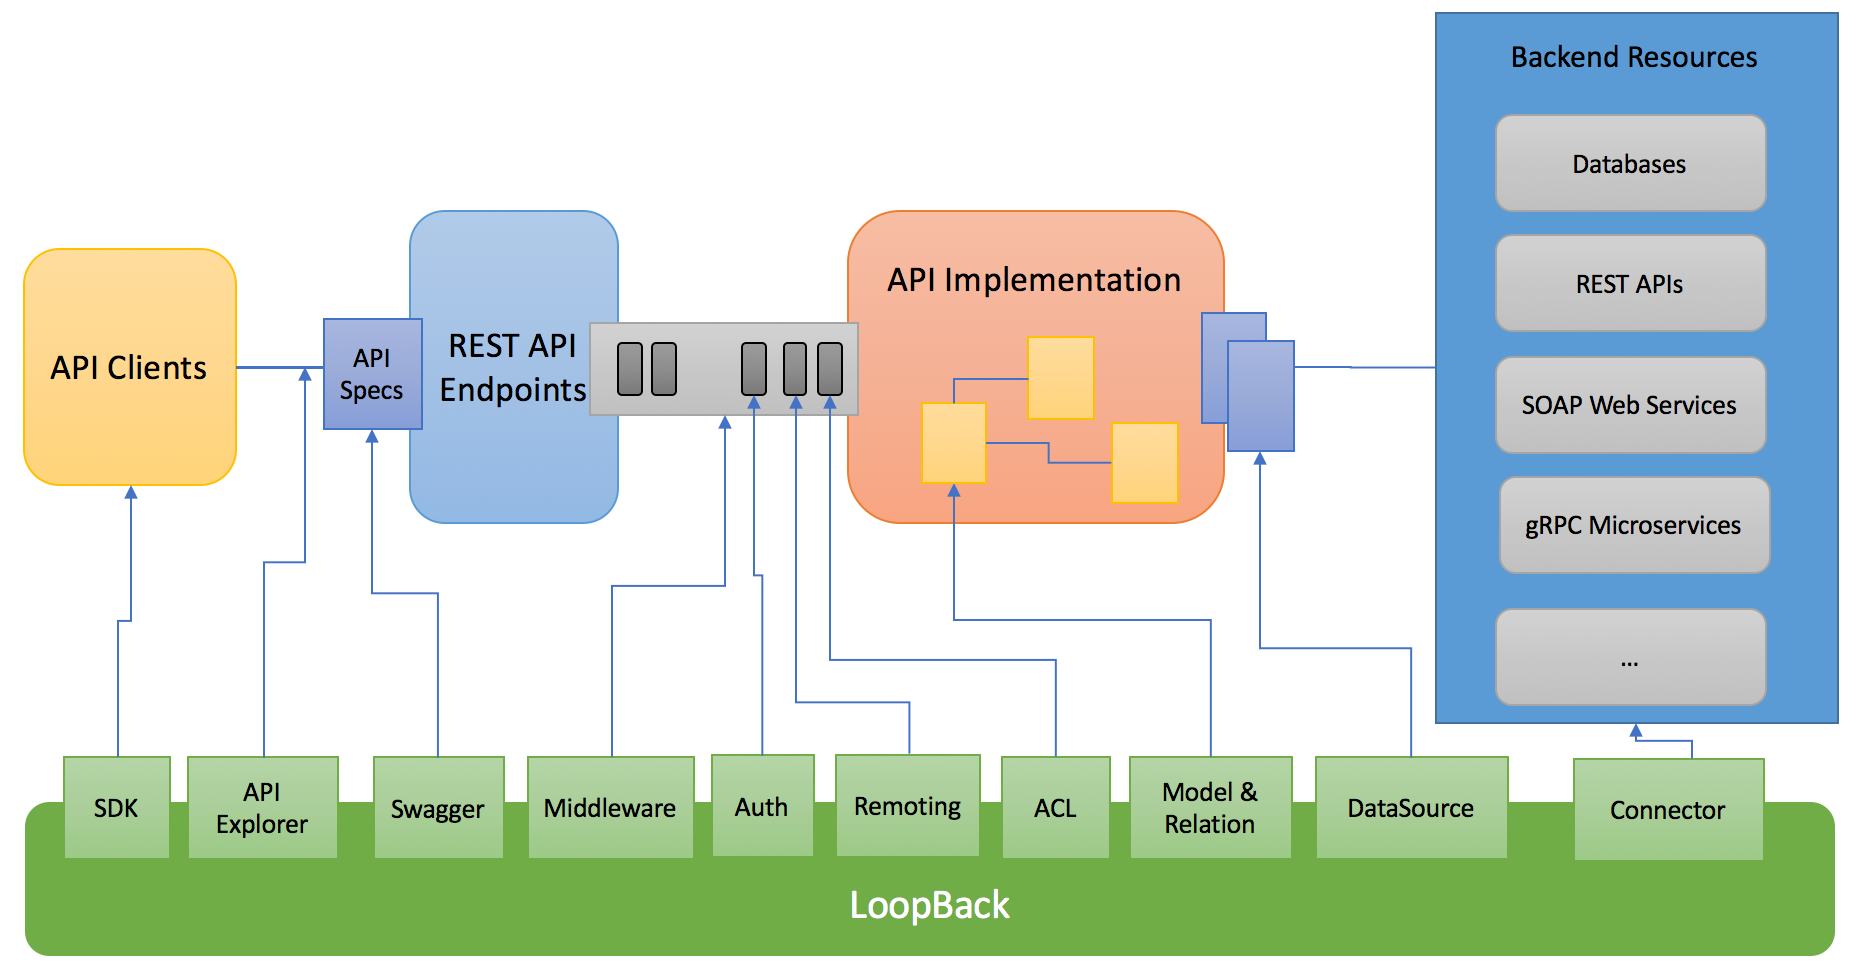
\includegraphics[scale=0.45]{lb4-overview.png}
    \caption[Loopback Architecture]{Loopback 4 Architecture}
    \label{implementation:fig:loopbackarchitecture}
\end{figure}

\paragraph{MoongoDb Datasource}
In the backend implementation using LoopBack 4, we used a MongoDB database as the data source for our application. 
LoopBack 4 provides an easy way to create and configure data sources using its \ac{cli}.
We used the \ac{cli} to generate a MongoDB data source for our application by running the command \texttt{lb4 datasource}. 
It generated a data source file (see Listing \ref{listing:implementation:lb4Mongo}) with the necessary configuration for connecting to our MongoDB instance.
We customized the data source configuration to include the database name and other options, such as the connection string, username, and password in an env variable \texttt{DB\_CONNECTION}.

\begin{lstlisting}[language=JavaScript, caption=lb-4-mongo.datasource.ts, label=listing:implementation:lb4Mongo]
// imports ...

const config = {
  name: 'mongo',
  connector: 'mongodb',
  url: process.env.DB_CONNECTION,
  useNewUrlParser: true
};

// Observe application's life cycle to disconnect datasource when application is stopped
@lifeCycleObserver('datasource')
export class MongoDataSource extends juggler.DataSource
  implements LifeCycleObserver {
  static dataSourceName = 'mongo';
  static readonly defaultConfig = config;
    
  constructor(@inject('datasources.config.mongo', {optional: true})
       dsConfig: object = config) {
    super(dsConfig);
  }
}
\end{lstlisting}

\paragraph{REST Controller}
Using Loopback 4, we created RESTful APIs for our application. 
The REST controller was generated using the LoopBack \ac{cli} tool, which provided a boilerplate code structure for creating REST endpoints.
To connect the REST controller to our application's business logic, we connected it to the repository and services. 
It allowed us to define the operations that could be performed on the model and provide implementation details.
We also implemented APIs for file uploads (see the Listing \ref{listing:implementation:fileUpload}), specifically CSV files and images, necessary for our prototyping tool. 
We created a function called \texttt{fileUpload}, which takes in a \texttt{@requestBody} containing the file to be uploaded. 
This function used the Nginx File input module to process file upload. 
Once the file is uploaded, we save it to our server folder.

\begin{lstlisting}[language=JavaScript, caption=file-upload.controller.ts, label=listing:implementation:fileUpload]
// imports ...
export class FileUploadController {
    constructor(...) {}
    
    @post('/files/{key}', {
        responses: {...},
    })
    async fileUpload(
        @requestBody.file()
        request: Request,
        @inject(RestBindings.Http.RESPONSE) response: Response,
        @param.path.string('key') key: string,
    ): Promise<object> {
        this.handler(request, response, async (err: unknown) => {
        this.uploadCsv(files["files"][0]["path"], key)
        })
    }

    private uploadCsv(file: File) {
        ...
    }
}
\end{lstlisting}

\paragraph{Model for data}
In our implementation, we used the CLI to generate our models.
A data model in Loopback is essentially an entity representing a collection of data or a resource. It can have various properties that define its schema, such as the data type, validation rules, default values, etc.
In our implementation, we defined our data model with various properties (as shown in Listing \ref{listing:implementation:datamodel}) like \texttt{id} of type \textit{string}, \texttt{key} of type \textit{string}, an \textit{array} of \texttt{data} and some other properties.
We also defined validation rules and default values for some of these properties.
Overall, a model in Loopback 4 provides a structured way of organizing and storing data in our application.

\paragraph{Other components}
We implemented a \textit{Middleware} using the \texttt{@authenticate(`jwt')} decorator to secure the API endpoints and authenticate the user. 
This decorator validates the JWT token sent in the request header and authenticates the user based on the token's validity. 
If the token is valid, the user can access the endpoint; otherwise, a \texttt{401} unauthorized error is returned.
\textit{OpenAPI} is a specification that allows developers to define, create, and consume RESTful APIs. 
We used the Loopback OpenAPI specification to generate API documentation for our application. 
The OpenAPI specification defines the API's endpoints, parameters, request and response bodies, and authentication requirements. 
The specification generates interactive documentation, client libraries, and code snippets to help developers integrate with the API. 
We configured the OpenAPI specification by defining the application's metadata, security schemes, and endpoints in the Loopback configuration file.
Finally, we used a predefined docker file generated from the Loopback CLI to deploy the application. 
The file specified the base image, environment variables, exposed ports, and dependencies required to run the application. 
The docker file contained all the necessary instructions to build and run the application in a containerized environment.

\begin{lstlisting}[language=JavaScript, caption=data.model.ts, label=listing:implementation:datamodel]
@model({ settings: { strict: false } })
export class DataModel extends Entity {
    @property({
        type: 'string',
        id: true,
        generated: true
    })
    id?: string;

    @property({
        type: 'string'
    })
    key?: string;

    @property({
        type: 'array',
        itemType: 'object',
        required: false,
        default: []
    })
    data: any;

    [prop: string]: any;

    constructor(data?: Partial<DataModel>) {
        super(data);
    }
}
\end{lstlisting}
\clearpage

\section{Database Schema}
\label{implementation:section:database}
In our database implementation, we used MongoDB as our database, which is a non-relational database system. 
MongoDB is a NoSQL database management system that uses a document-oriented data model. It is designed to scale horizontally across many servers, making adding new nodes to an existing cluster easy to increase capacity and improve performance.

\begin{figure}[ht]
    \centering
    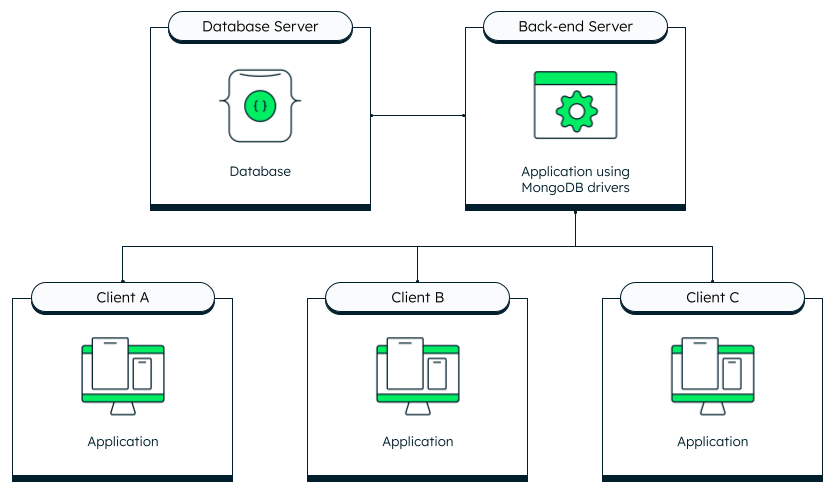
\includegraphics[scale=0.5]{mongo-architecture.png}
    \caption[MOngoDB Architecture]{Peer-to-peer architecture of our MongoDB implementation}
    \label{implementation:fig:mongoarchitecture}
\end{figure}

MongoDB follows a peer-to-peer architecture (see figure \ref{implementation:fig:mongoarchitecture}\footnote{Website for MongoDB architecture: \url{https://www.mongodb.com/basics/database-architecture}}), where each node can act as a client, server, or both, and nodes can communicate directly.
Our implementation architecture includes using MongoDB Atlas, a cloud-based service for managing MongoDB databases. It allows us to easily manage and scale our database with features such as automatic scaling and backups.
The data is stored in a collection of documents, which can be considered similar to rows in a traditional relational database. Each document consists of a set of key-value pairs and can have a flexible schema, allowing for dynamic data structures. It is in contrast to a traditional relational database with a fixed schema.
We have implemented a 3-tier architecture for our application, with the frontend, backend, and database layers. Using JavaScript code allows us to perform CRUD (Create, Read, Update, Delete) operations on the database.

We created two main tables, \textit{View} and \textit{Experiment} (see figure \ref{implementation:fig:erdb} containing the Entity Relationship diagram), to store the data for our prototype and experimentation phases. 
The first table we created is called \textit{View} and is used to store the various UI screens in our application for the prototyping section. 
The \textit{View} table in our database schema is a crucial component of the prototyping feature. 
It stores various UI screens with properties like \textit{ID, Name, property, elements, and children}. 
The ID and Name are both strings and ID is used for uniquely identifying each view. 
The \textit{property} is a JSON object storing different properties like CSS properties, screen dimension properties, etc. 
Similarly, the \textit{elements} property persists an array of UI elements that are part of that view. 
These UI elements have properties like \textit{ID, Name, cssProperties, interactions}, etc.

\begin{figure}[ht]
    \centering
    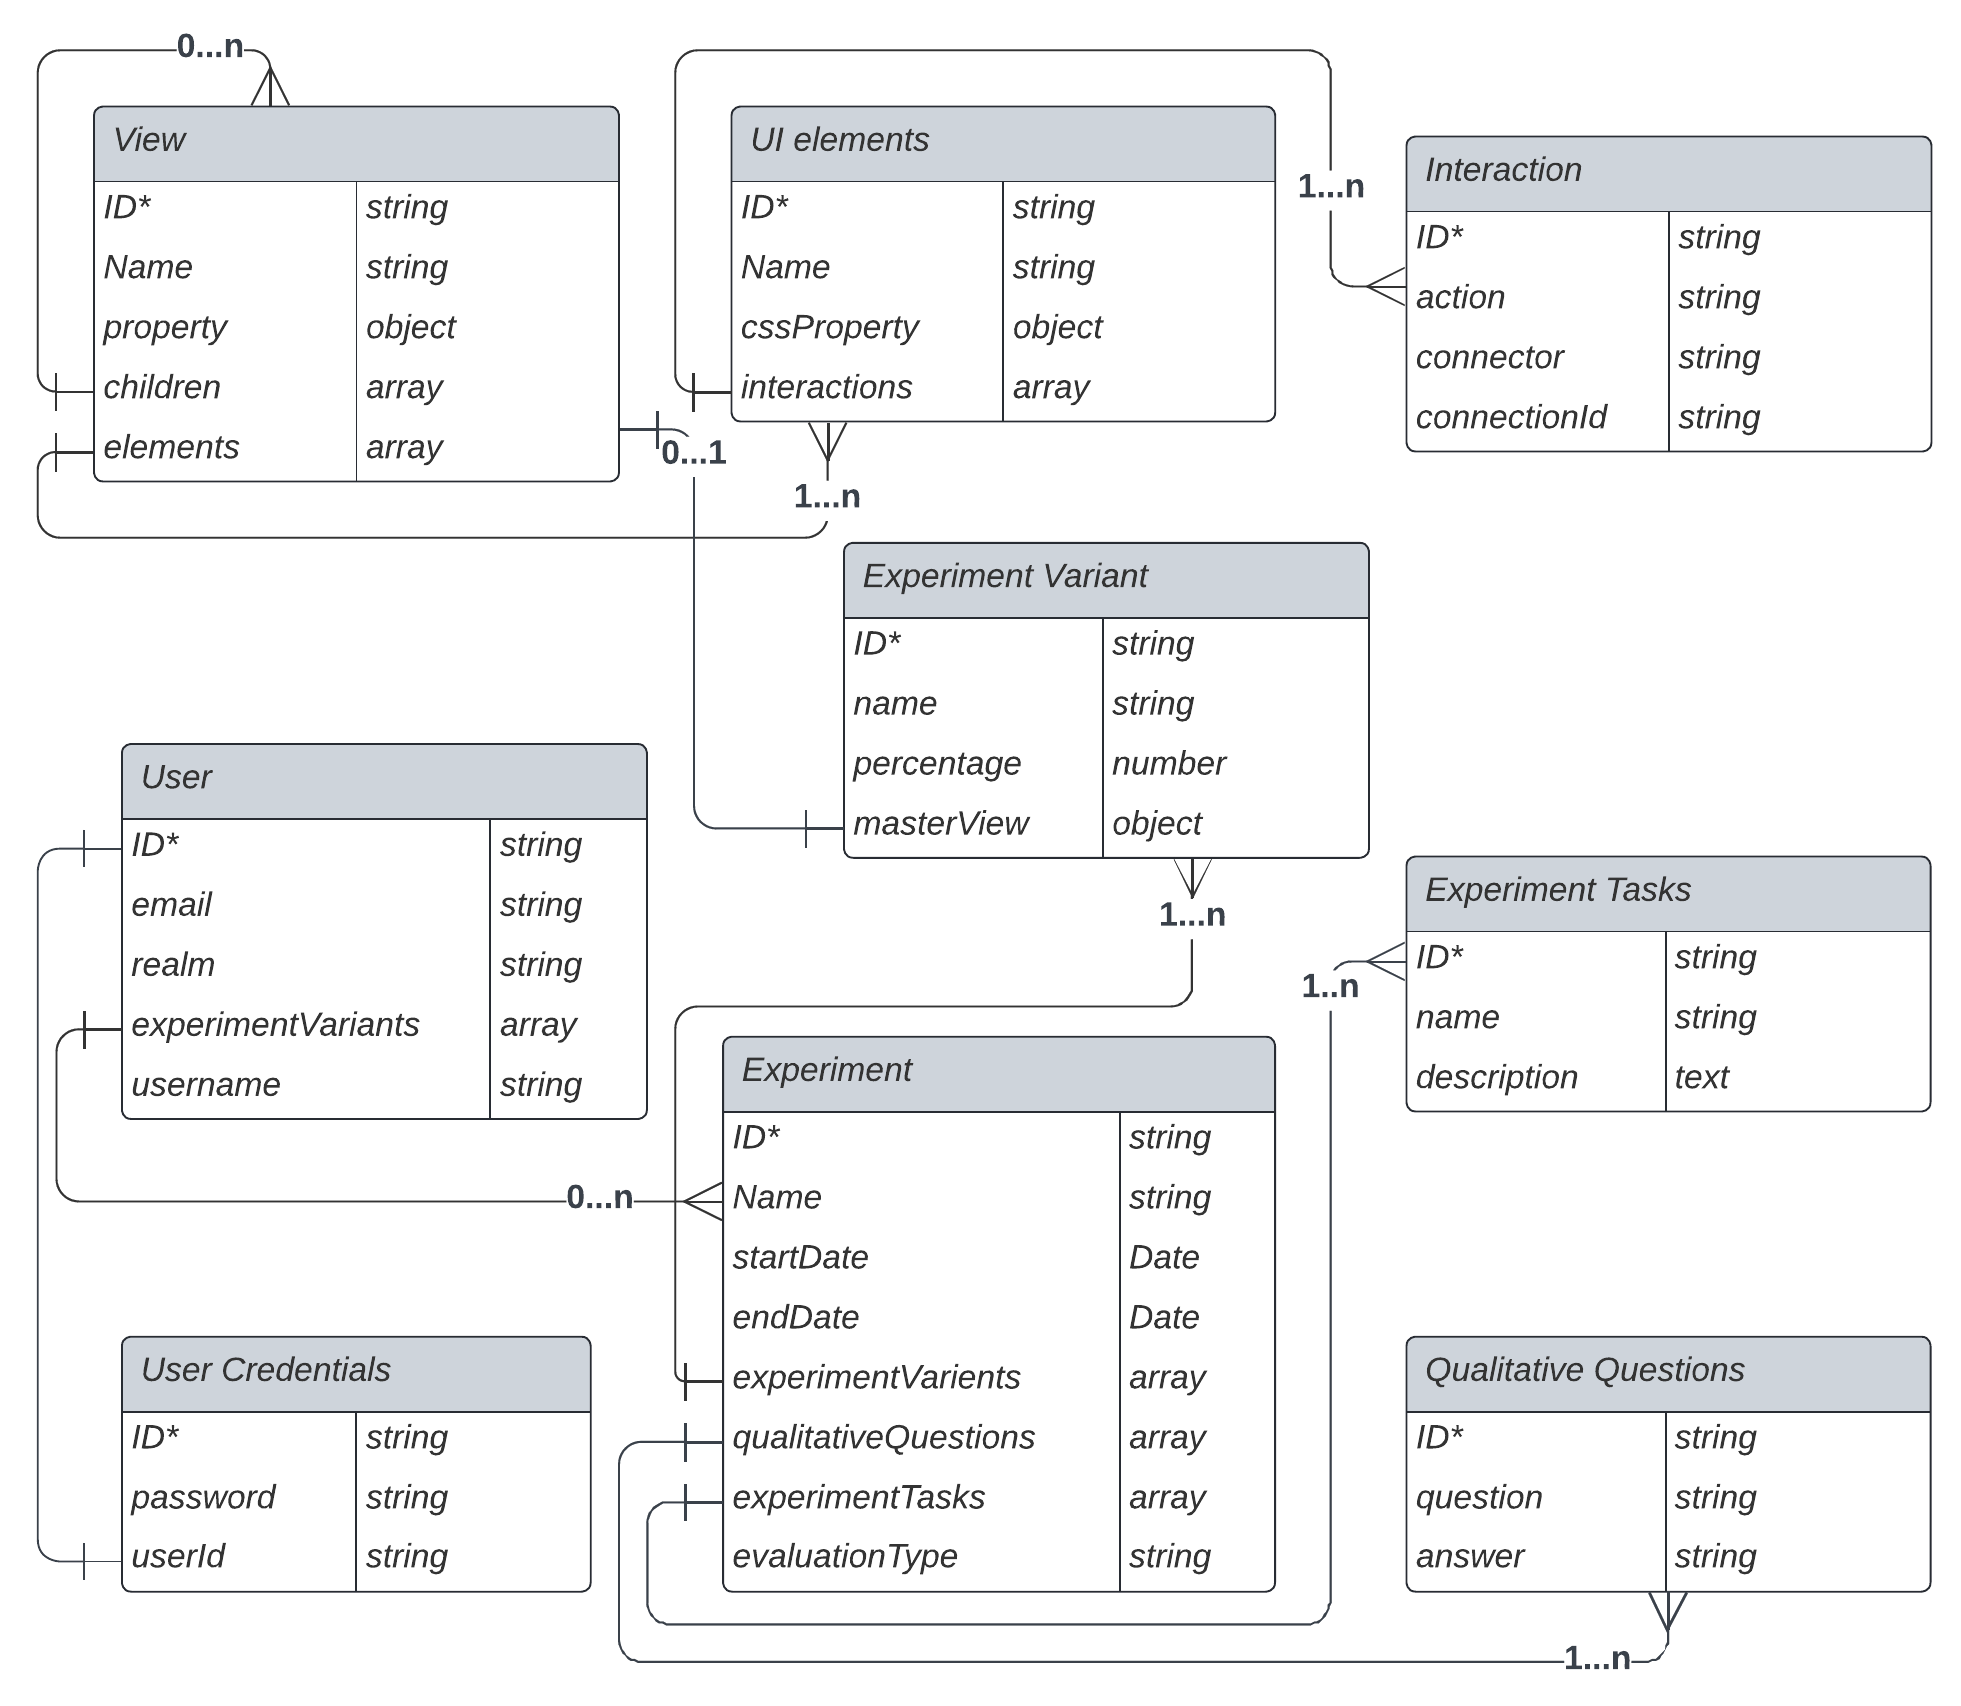
\includegraphics[scale=0.22]{ER-diagram.png}
    \caption[ER Diagram]{Entity Relation Diagram of the Tool}
    \label{implementation:fig:erdb}
\end{figure}

Furthermore, the \textit{View} table also contains the \textit{children} property, which stores an array of \textit{Views}. 
It's a cyclic reference, allowing us to create complex views by nesting views within each other. 
For instance, a parent view might contain two child views, each with unique UI elements and properties.
By storing this information in the \textit{View} table, our application can easily retrieve all the necessary information to render the UI, including the properties of each UI element and how they relate to each other in the view hierarchy. 
This information is crucial for the prototyping feature as it allows users to create and visualize complex UI designs.

The second table in our MongoDB database schema is the \textit{Experiment} table. 
This table stores details related to the experiment and contains properties such as \textit{ID, Name, startDate, endDate, experimentTasks, qualitativeQuestions, experimentVariants, and evaluationType}.
The ID and Name are both strings and the ID is used for uniquely identifying an experiment in the database. 
The \textit{startDate} and \textit{endDate} properties are used to store the dates between which the experiment was conducted.

The \textit{experimentTasks} property is an array of experiment tasks to be performed as part of the experiment. 
Each task has a unique ID, a name, and a description.
Similarly, the \textit{qualitativeQuestions} property is an array of qualitative questions to be answered by the participants after completing the experiment. 
Each question has a unique ID, a question, and an answer.
The \textit{experimentVariants} property is an array of experiment variants to be used. 
Each variant has a unique ID, a name, and a percentage. The \textit{percentage} property is used to specify the percentage of participants assigned to the variant. 
Additionally, each variant is associated with a \textit{masterView}, a \texttt{View} entity representing the prototype of the user interface for that variant.
Finally, the \textit{evaluationType} property is used to specify the type of evaluation that will be performed for the experiment.

In addition to the \textit{View} and \textit{Experiment} tables, our database schema also includes a \textit{User} table for storing user information with different user roles such as admin, participant, etc. 
This table contains properties such as \textit{ID, email, realm, username, and experimentVariants}.
The \textit{ID} property serves as the unique identifier for each user, while \textit{email} and \textit{username} store the user's email and username, respectively. 
The \textit{realm} property stores the user role assigned to the user, and \textit{experimentVariants} is an array of experiments assigned to the user, precisely the variant of the experiment assigned to the participant.
By storing this information in the database, we can keep track of user information and their assigned experiment variants. 
This information is used in the experiment to ensure that participants are assigned to the correct experiment variant and that their responses are recorded accurately. 
Finally, the \textit{User} table plays a critical role in our application by ensuring that user information is stored accurately and can be easily accessed and managed.

Overall, our database implementation allows us to store and manage complex hierarchies of UI screens and interactions and store data related to our experimentation phase.